%!TEX root = karen.tex

\chapter{Neighbor Queries and Node Ordering}


\section{Neighbor Queries} 

As part of the preprocessing stage for RBF-FD, the scattered point cloud must be analyzed to generate stencils. To generate a stencil, any collection of nodes can be selected. However, by choosing nodes close to the stencil center and well balanced around it, we stand to get the best possible approximations to derivatives. 

Why? well, the approximations are based on differences. Similar to classic FD, draw a secant connecting two nodes of a stencil. The slope of the secant determines the gradient at either point or a point in between. In the limit as the points are moved closer to the same spot, the approximation to the derivative at that point becomes exact. 

So ideally every RBF-FD stencil will operate on nearest neighbors. One way to generate nearest neighbors is brute force $O(N^{2})$; very inefficient. 

Alternatives exist including k-D Tree

\subsection{k-D Tree}
Build complexity, seek times. Internal ordering 

We use implementation provided by Andrea Tagliasacchi \cite{tagliasacchi} as a MEX compiled set of routines for Matlab. These same routines are then linked into C/C++. 

\subsection{Locality Sensitive Hashing}

\cite{Connor2009} provide a fast parallel 

\cite{Henke2012} is working on parallel generation. \cite{IanJohnsonThesis} has OpenCL neighbor queries

We started with a CPU implementation to test appropriateness. 

\authnote{Compare performance of stencil generation in C++}

\begin{figure}
\centering
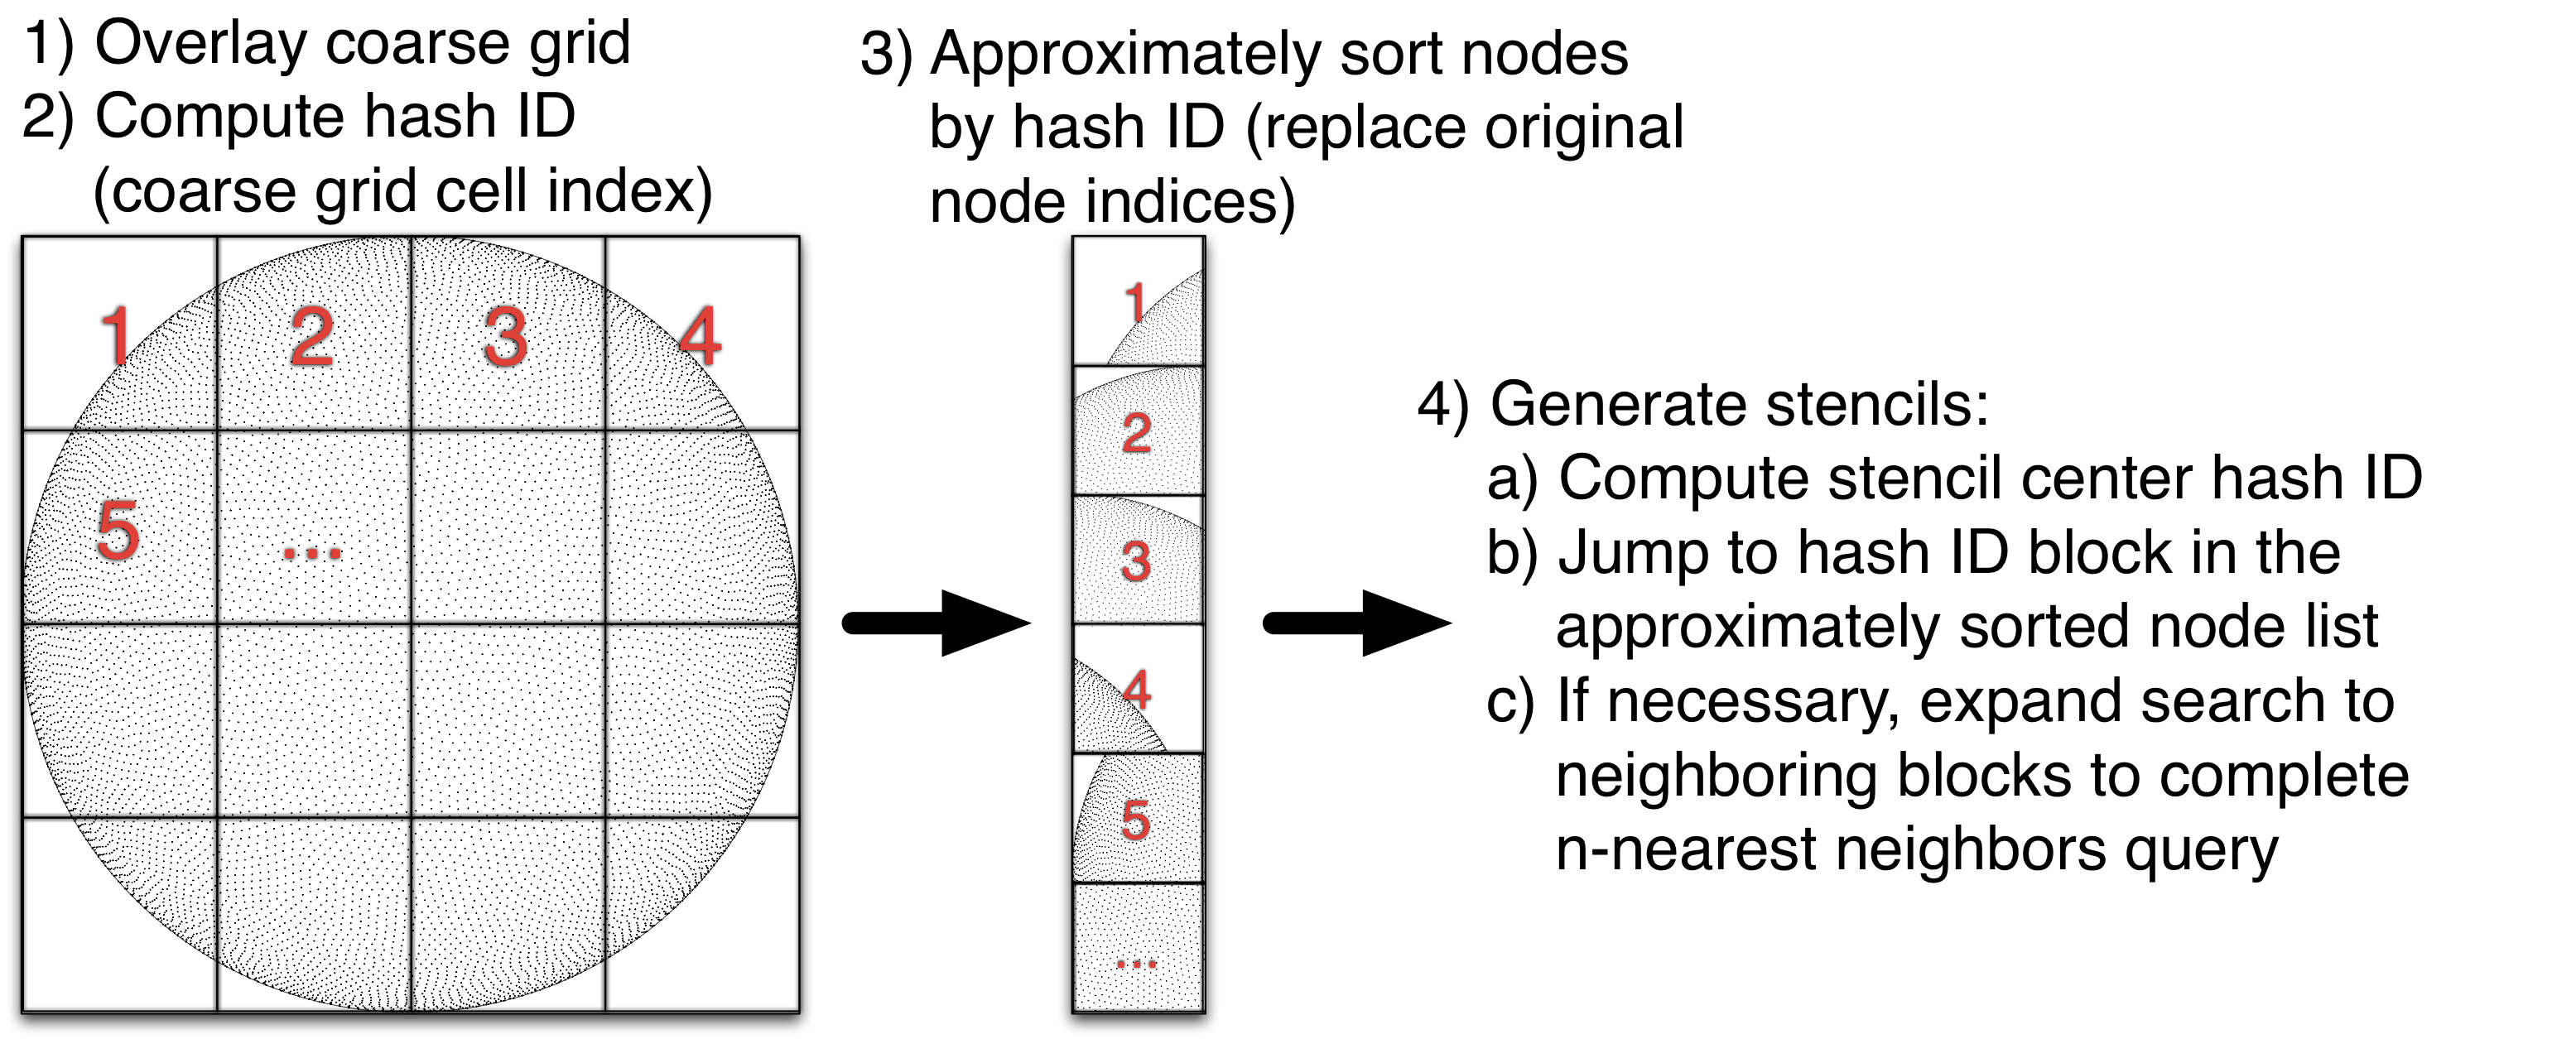
\includegraphics[width=1.0\textwidth]{figures/chapter7/LSH_Concept.pdf}
\caption{High level overview of Locality Sensitive Hashing algorithm. First we overlay a coarse regular grid on the bounding box of the domain. The cells of the coarse grid cells are reordered in memory according to a space filling curve. Then we query neighbors by starting search with \authnote{Illustrate the query process} cell containing stencil center and append neighboring cells until stencil size $n$ nodes are found. We take $n$ closest neighbors (brute force search) if more than $n$ are appended to the list of candidates. }
\end{figure} 

\begin{figure}
\centering
\begin{subfigure}{0.425\textwidth}
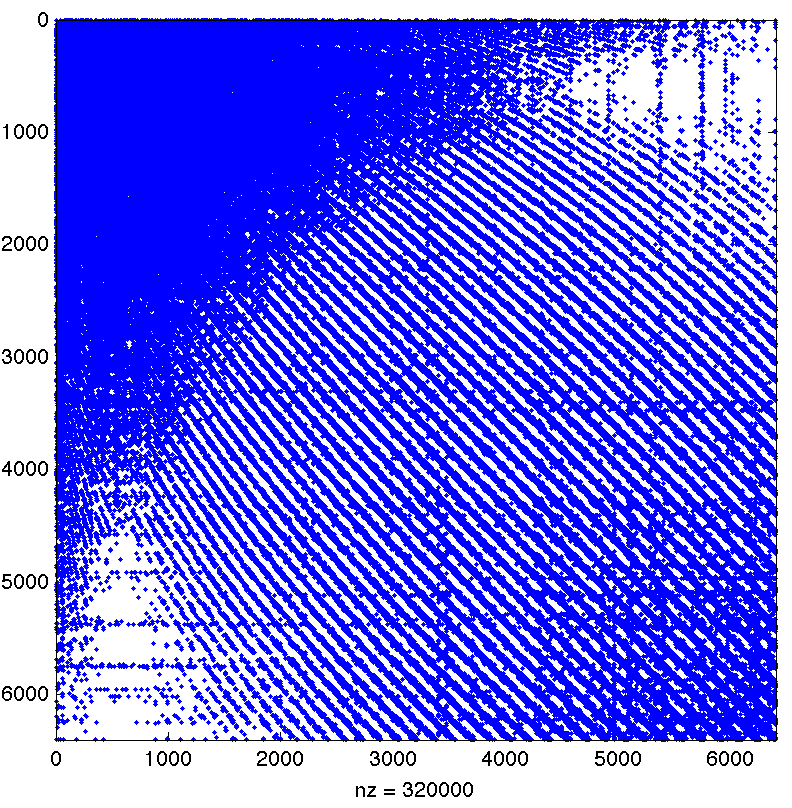
\includegraphics[width=1.0\textwidth]{figures/chapter7/bruteforce_N6400_n50.pdf}
\caption{k-D Tree} 
\end{subfigure} 
\begin{subfigure}{0.425\textwidth}
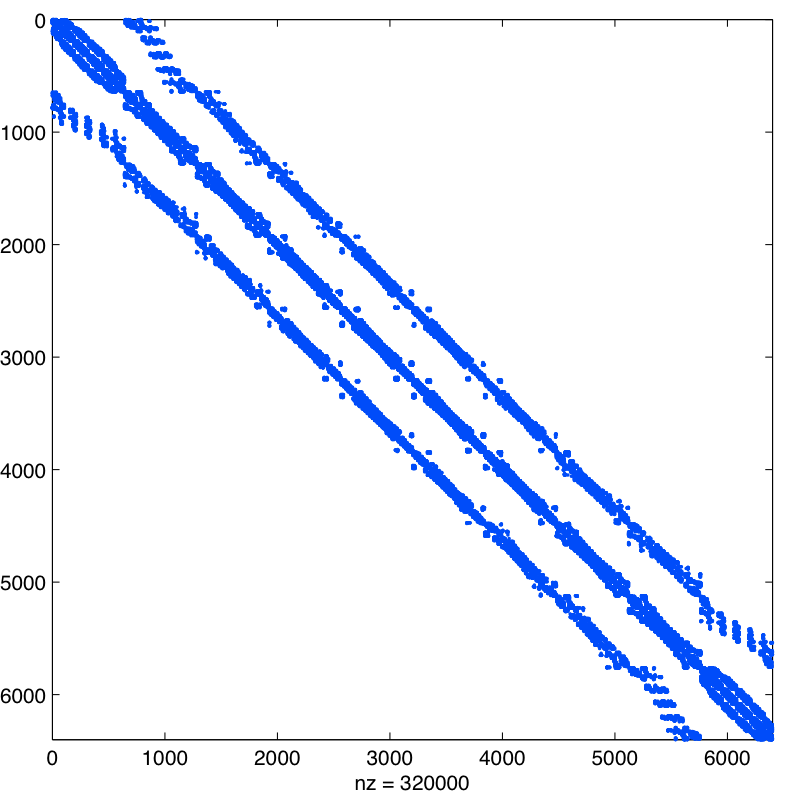
\includegraphics[width=1.0\textwidth]{figures/chapter7/lsh_N6400_n50.pdf}
\caption{LSH}
\end{subfigure}
\caption{Example effects of node reordering within neighbor query algorithm for MD node set $N=6400$ with $n=50$. Matrix is $0.78\%$ full. k-D Tree maintains original ordering of the nodes and deceptively appears nearly dense. LSH algorithm reorders nodes according to raster ordering and reveals sparsity of the problem.  }
\end{figure} 

\section{Node Ordering}

Locality sensitive hashing also allows us to reorder the nodes

\cite{Saad2003} mentions the impact of ordering on conditioning.

Algorithms like Reverse Cuthill McKee and Approximate Minimum Degree ordering allow general restructuring of matrices. 

\authnote{NEed to compare conditioning of LSH and other algorithms in Matlab}

Q: what is an ideal ordering?
Q: what is the best conditioning from ordering?
Q: what is the relative cost of ordering?


